\documentclass{article}

% if you need to pass options to natbib, use, e.g.:
% \PassOptionsToPackage{numbers, compress}{natbib}
% before loading nips_2018

% ready for submission
%\usepackage{nips_2018}

% to compile a preprint version, e.g., for submission to arXiv, add
% add the [preprint] option:
\usepackage[preprint]{nips_2018}

% to compile a camera-ready version, add the [final] option, e.g.:
%\usepackage[final]{nips_2018}

% to avoid loading the natbib package, add option nonatbib:
% \usepackage[nonatbib]{nips_2018}

\usepackage[utf8]{inputenc} % allow utf-8 input
\usepackage[T1]{fontenc}    % use 8-bit T1 fonts
\usepackage{hyperref}       % hyperlinks
\usepackage{url}            % simple URL typesetting
\usepackage{booktabs}       % professional-quality tables
\usepackage{amsfonts}       % blackboard math symbols
\usepackage{nicefrac}       % compact symbols for 1/2, etc.
\usepackage{microtype}      % microtypography
\usepackage[super]{nth}     % JK: for 1st-ing and 2nd-ing

\usepackage{graphicx}       % added by seth - image support
\graphicspath{ {./images/} }
\usepackage{soul}           % added by seth - remove before submission, provides highlighting support
\usepackage{wrapfig}        % added by seth for placing images in-line with text

\usepackage{hyperref}
\hypersetup{
    colorlinks=true,
    linkcolor=blue,
    filecolor=magenta,
    urlcolor=blue,
}
 
\urlstyle{same}
\title{%
  Kung Faux Pandas \\
  \large Simplifying privacy protection
  }

\author{
  James King, Seth Russell, Tellen D. Bennett, Debashis Ghosh\\
  Data Science to Patient Value (D2V)\\
  School of Medicine\\
  University of Colorado Anschutz Medical Campus\\
  Aurora, CO\\
  \texttt{\{james.king, seth.russell, tell.bennett, debashis.ghosh\}@ucdenver.edu}
  }

\date{May 2018}

\begin{document}

% Advice from Tell:  articulate the problem with evidence (i.e. papers)
%   Enable reproducibility - patient value, make process of replication easier
%   Time saving
%   legal risk (carrying data in laptops, etc)
%   Multiple comparison?
%   Educational data sets
%  Definition of :reproducibility 
%       reproducibilty - everything same - code, data, result
%       replicability - code same, new data, same result find Peng & Leek reference (also look at blog)
%   unit testing...
%   Proof of privacy guarantees?

\maketitle

% this tool simplfies data sharing, simplifies data exploration within organizations
\begin{abstract}
Kung Faux Pandas is an end-to-end system for easily generating synthetic data that is statistically similar to real data but lacks sensitive information. This publicly available \footnote{\url{https://github.com/CUD2V/kungfauxpandas}} system lowers barriers to HIPAA- and GDPR-compliant data sharing for reproducibility testing and other purposes.
\end{abstract}


\section{Introduction}

Independent reproduction and replication of results are critical components of scientific inquiry. Barriers to data access and sharing are the most important impediments to reproducibility in computational research. Health care research has unique challenges because of necessary personal data privacy protections.

Several methods exist to de-identify (remove key identifiers, group individuals, and related anonymization techniques \cite{hippapro}) and synthesize data (create data through algorithmic means, population level statistics, randomization, ideally with preservation of multivariable relationships between records \cite{walonoski_synthea_2018, patki_synthetic_2016, choi_generating_2017}). However, no pipeline currently exists with which computational investigators can routinely \emph{anonymize} or \emph{synthesize} data to facilitate access and sharing. This work addresses that gap.

We have created an open source software library called \emph{Kung Faux Pandas (KFP)} which allows for the modular combination of established privacy protection methods with the popular Python Pandas data science library\cite{mckinney-proc-scipy-2010}. KFP also provides a Structured Query Language (SQL) interface which enables users to query a database and receive a data set without personal information through either anonymization or synthetic data generation. 

\section{Background}

% shorten this? Is this the right place in the background for this?
Recent work has clarified the definition and importance of reproducibility and a closely related entity, replicability. Leek and Peng have defined reproducibility as the "ability to recompute data analytic results given an observed dataset and knowledge of the data analysis pipeline," and replicability as "the chance that an independent experiment targeting the same scientific question will produce a consistent result."\cite{leek_opinion_2015,peng_reproducible_2006} Others have used the terms in a reverse fashion.\cite{drummond_replicability_2009} Despite the semantic differences, there is broad agreement that an independent experiment with confirmatory results is the strongest support of any experiment. One early influential paper on the topic of reproducibility in scientific computing lists the key factors in reproducibility as available data, input parameters, documentation, software code, and an environment capable of running the provided software code. These items are difficult to completely convey in a traditional research paper \cite{schwab_making_2000}. 
In the context of machine learning (ML), sufficient detail is required such that an independent investigator could create the same hardware and software configuration, data used for all experiments, source code, documentation on data and how to run/configure software, and tests that verify the software runs correctly. Once a result can be reproduced, new researchers can then build upon the methods, gather new data for testing/validation, or discover alternative methods to replicate a result.

In the health care domain in the United States the key law governing health data is the Health Insurance Portability and Accountability Act (HIPAA). HIPAA is backed by significant civil penalties as well as specifics about security and what can and cannot be done with protected health information \cite{hippaviol}. There are two primary methods by which data can be shared or made public: de-identifcation, the removal of specific identifiers or summarization to a level at which individual identification is minimized, and through strict legal relationships called a business associate agreement. Even institutions which share data within the confines of the laws face a steep institutional risk. These legal barriers makes it difficult to enable independent verification of machine learning (ML) models which often require enormous amounts of training data.

Perhaps more ominously and broadly relevant for researchers, on May 25, 2018 the European Union's (EU) General Data Protection Regulation (GDPR) has come into full effect \cite{gdpr}. This law establishes a new paradigm in data ``ownership'' for that jurisdiction. This set of rules defines the ``owners'' of data to be people from whom it was collected and obliges anyone possessing that data to honor the owners' preferences about how the data is kept and used, including a requirement to deletion of any data at the request of its owner at any time in the future.

% continue re-writing from here
These rules are ultimately good for citizens, but they create a pickle for scientists studying humans as it's very difficult to follow normal processes in scientific rigor while complying with privacy protection rules.

% Logical step our work is taking. 
One obvious way around this pickle is to separate data and analysis in such a way that the analysis can be performed on data without the \emph{analyst} having access to the data. This is fairly straight-forward to implement. Essentially, the analyst, with only a description of the sensitive data, composes analytical code which is handed off to the data custodian. The custodian then runs it and returns the results to the researcher.

This has been technologically possible for some time, but it's awkward in practice because activities such as data cleaning, exploration, and plotting are interactive and iterative processes which would become impractical with a mediator.

% previously had some information about various data anonymization and synthesis techniques. Put that back?

\section{System Details}

% some text about goal to make our research reproducible/replicable - provide source code, pip/conda environment files, docker container
% explain why not full synthesize a full dataset. better to limit to sql query where relevant data is brought together; easier to model 1 table than lots of separate tables. Modelling lots of separate tables requires extensive meta data configuration and a significant amount of computing power to generate...
% where to put this text? "Unit testing is important but often overlooked - unit tests can show how a researcher validated their code was giving expected results which can often lead to insights not normally communicated in a results section of a journal article."

% What is our major contribution to the area of reproducibility in machine learning?
KFP sidesteps this problem by generating \emph{faux data} that is ``statistically similar'' to the real data but does not itself contain any sensitive data. We collectively refer to de-identified data and synthetic data as \emph{faux data}. We use the word faux in its standard sense of artificial or fake, but more specifically as it is used in fashion: man-made materials that look and feel like real leather, fur, etc., but wihout the problematic derivation from live animals and reliance upon limited resources.

% this is a key unique feature of this work and should likely be repeated in conclusion. Perhaps also include in abstract
This faux-data can be prodded, poked, plotted, and posted for the world to see, enabling analysts to develop their code using whatever means they prefer. When the analytical code is ready, it can then be sent to the data custodian to run on the real data.

Many methods of generating faux data exist, some with freely available software implementations. KFP provides a standard mechanism for ``wrapping'' any method into a ``plug-in'' which integrates the method with the Pandas data frame model. Three of these plug-ins are provided with full documentation for creating other plug-ins.

\subsection{System Architecture}

Ideally, a computational investigator can develop, test, and validate models using all available data. However, as discussed previously, regulatory limitations may prevent data access. Even with regulatory approvals, data access processes can be slow. Figure~\ref{fig:architecture} shows the novel architecture of KFP: data access through an intermediary that can synthesize data on-demand.

\begin{figure}[ht]
  \centering
  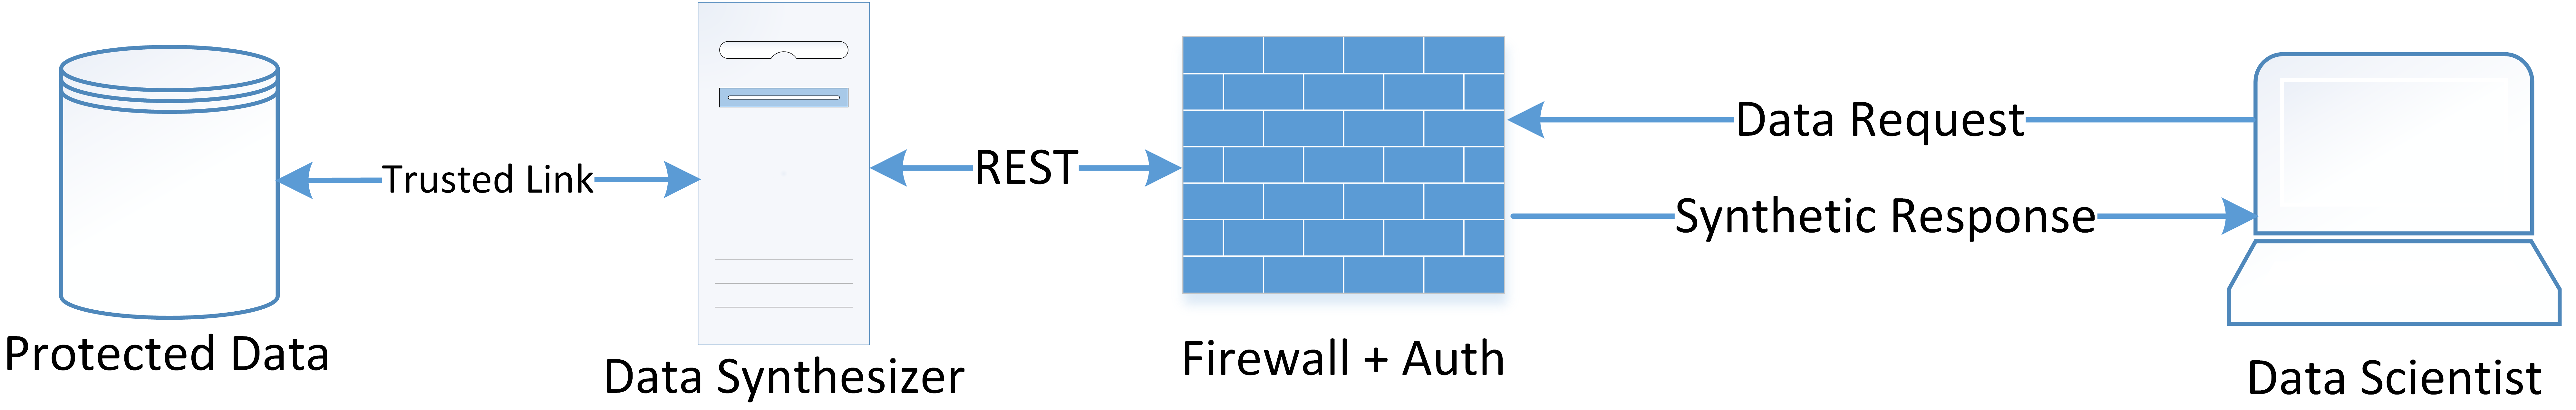
\includegraphics[width=\textwidth]{prototype_architecture}
  \caption{System Architecture.}
  \label{fig:architecture}
\end{figure}

Figure~\ref{fig:synthesis_process} shows the automated faux data request/response process. All queries submitted to the system are first pre-processed to remove clauses such as "ORDER BY" which are made ineffective by the synthesis process. All queries are logged for later analysis and results cached to optionally improve synthesis performance for repeated queries. Next the processed query is executed against the protected data set and results are passed into the modular synthesis process. While the current implementation only utilizes a couple of synthesis methods, ML developers or data warehouse owners can insert their own custom method or modify existing methods. Previously removed "ORDER BY" clauses are re-applied to the faux data before results are returned to the user. Finally, although not implemented in this version of KFP, synthetic results could be held back until reviewed and approved for release by the data owner.

% somewhere - here? Explain that the environment has been provided with a randomly generated dataset similar to one researchers have worked with during anlysis of a Sepsis prediction model.


\begin{figure}[ht]
  \centering
  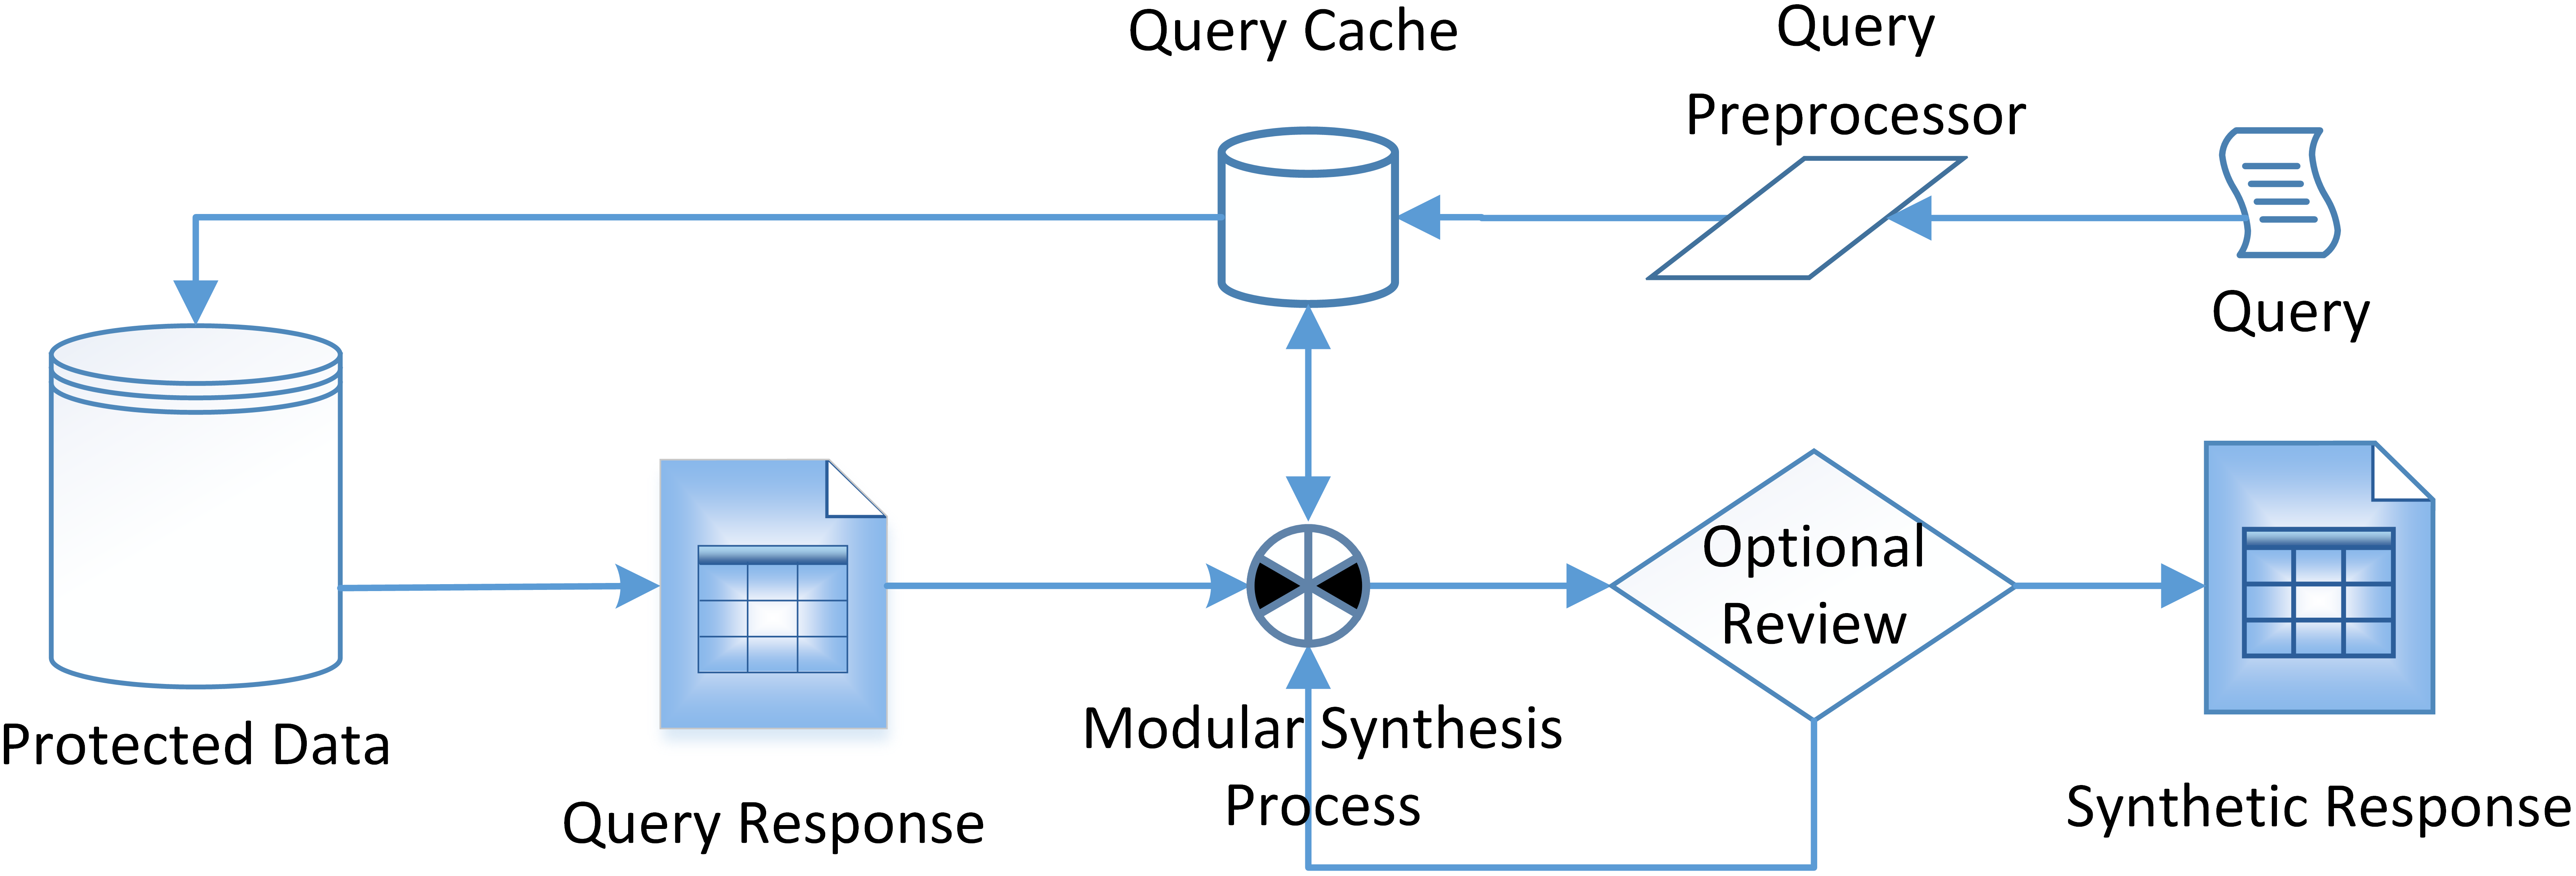
\includegraphics[width=120mm]{data_synthesis_process}
  \caption{Data synthesis process.}
  \label{fig:synthesis_process}
\end{figure}


\begin{wrapfigure}[15]{r}{0.5\textwidth}%optionally place [15] after {wrapfigure} to control how many lines to wrap around figure
  \centering
  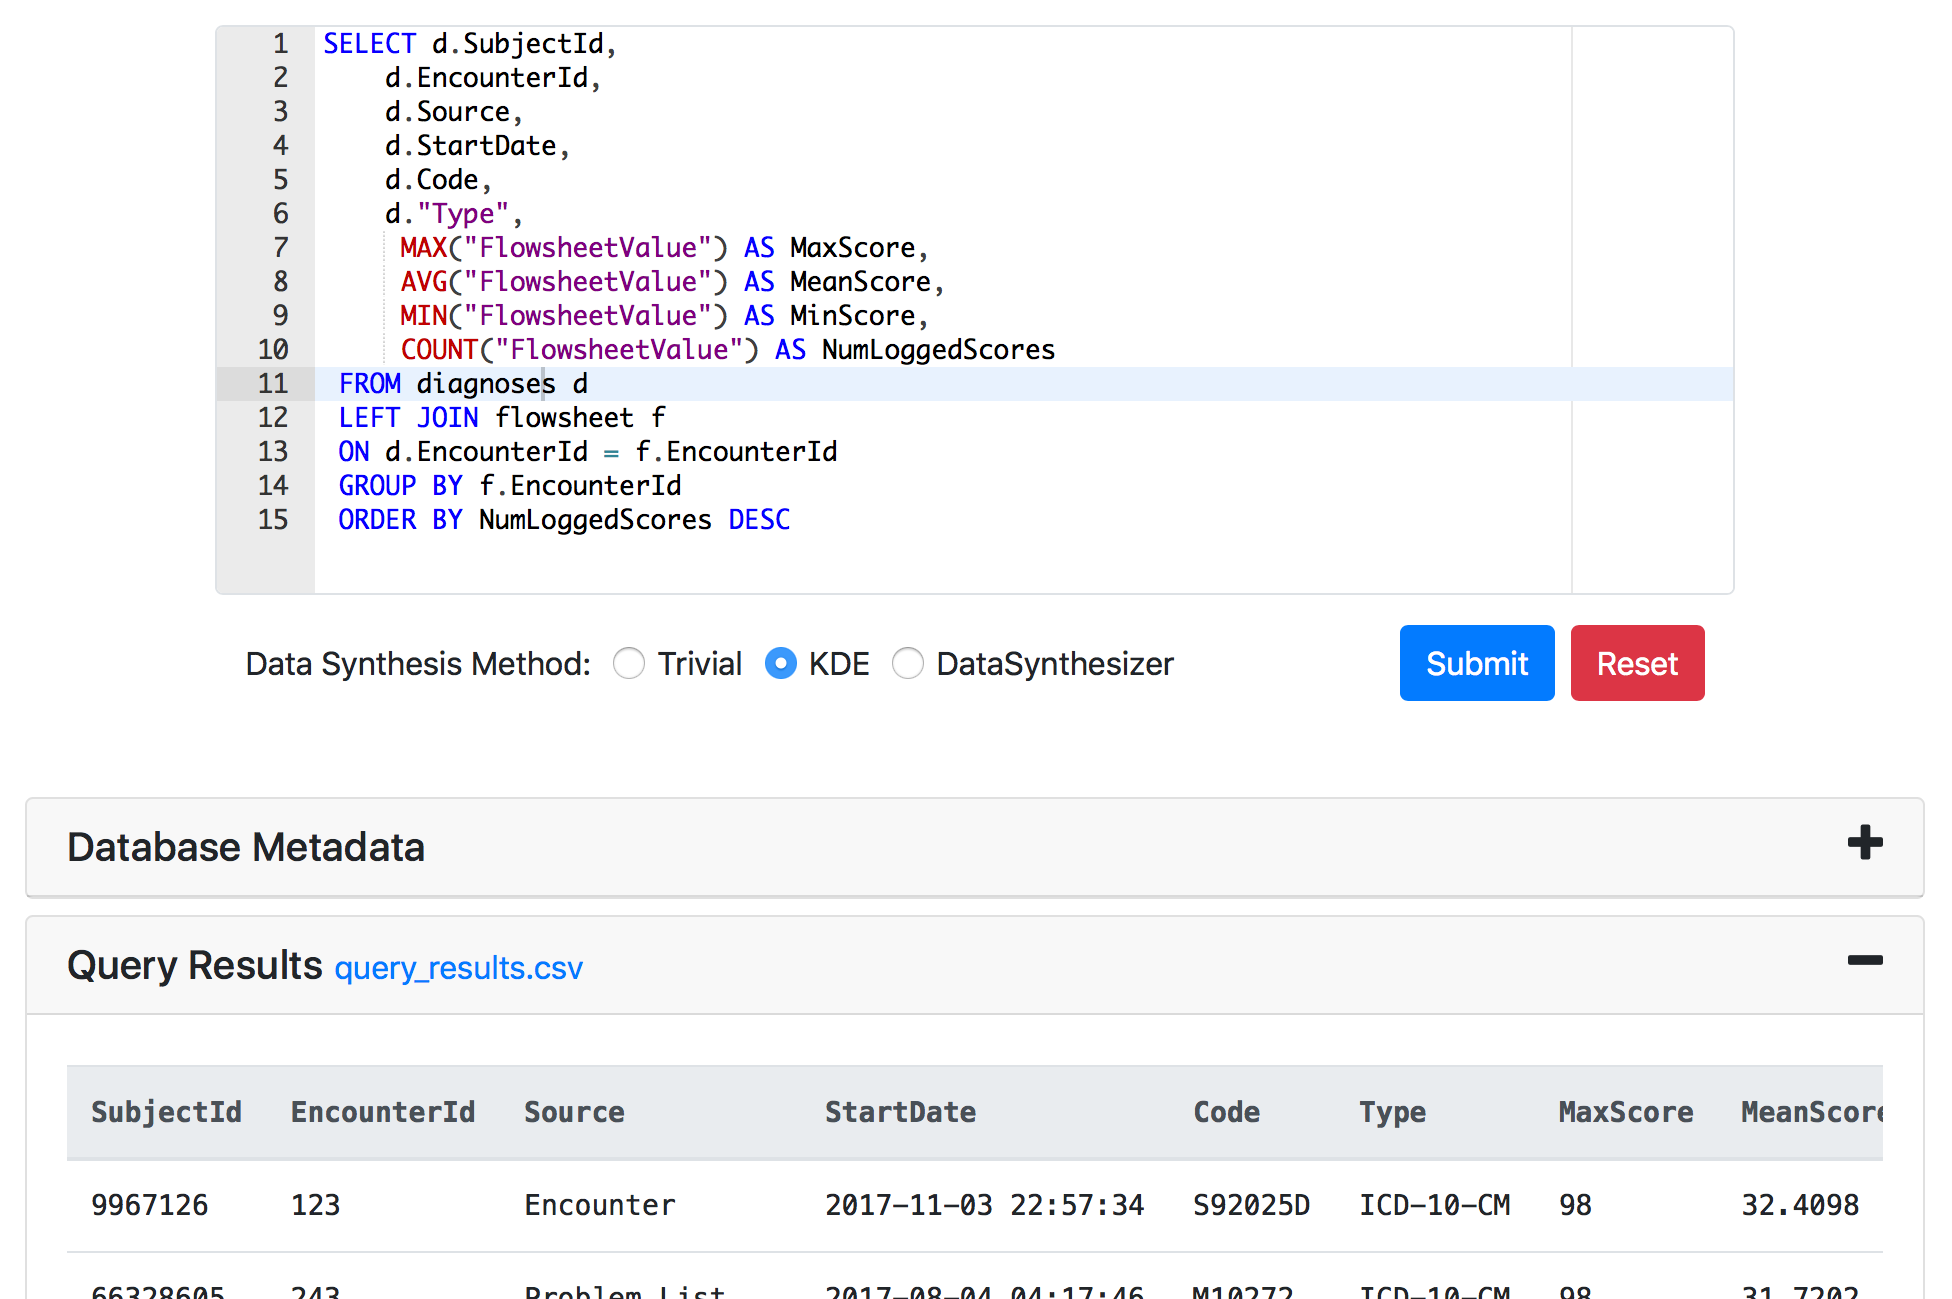
\includegraphics[width=0.5\textwidth]{ui_screenshot3}
  \caption{User Interface.}
  \label{fig:ui}
\end{wrapfigure}
KFP provides multiple methods by which a ML developer can access on-demand faux data. As shown in Figure~\ref{fig:ui}, a single page web application (SPA) allows for users to directly enter SQL queries, submit them to the connected database, and receive faux data according to the selected generation method. Data can either be viewed directly in browser or downloaded in csv format for use in a ML process. Alternatively, an http REST service (utilized by the SPA) allows for cross language compatible requesting and receiving of faux data, again via SQL query. In order to facilitate querying and understanding of the data model, the database metadata is presented to the user in a collapsible section. Lastly, for Python based software or languages with an interface to Python, the kungfauxpandas.py file and associated classes can be imported and called natively.

\subsection{Included Synthesis Methods}

KFP provides a framework by which any number of methods for data privacy can be carried out. For demonstration purposes we have implemented three plugins that use different techniques for data synthesis, as shown in Table~\ref{included-methods}. The kernel density estimator from scipy.stats.gaussian\_kde uses the method developed by Silverman \cite{silverman_density_1986} which handles inter-related ordinal and ratio data yet runs quickly on standard consumer level hardware. The DataSynthesizer method, created by Ping et al. \cite{ping17datasynthesizer} is built on differential privacy mechanisms and has multiple internal methods for data generation ranging from random generation based on data type to Bayesian modeling of inter-relationships among columns of data. Lastly, the Synthetic dataset Generation Framework (SGF) by Bindschaedler et al. \cite{Bindschaedler2017} "generates differentially private synthetic data" using a novel criterion called plausible deniability that is applied to a dataset before it is deemed safe to release. For SGF and DataSynthesizer, their authors show that the synthetic data generated preserves privacy while still being useful enough for actual data analysis (see also \cite{howe_synthetic_2017}). In the case of SGF, several models are built with both real and synthetic data and compared against a gold standard. Their author's analysis showed that the models from synthetic data are close to the same accuracy as models built with real data.

\begin{table}
  \caption{Kung Faux Pandas data synthesis methods}
  \label{included-methods}
  \centering
  \begin{tabular}{p{12em} l p{14em}}
    \toprule
    Method                                                 & Notes \\
    \midrule
    Kernel Density Estimator\cite{silverman_density_1986}              & Inter-related ordinal and ratio data\\
    DataSynthesizer\cite{ping17datasynthesizer}                                 & Bayesian modeling of column relationships\\
    Synthetic Generation Framework\cite{Bindschaedler2017}      & Probabilistic modeling\\
    \bottomrule
  \end{tabular}
\end{table}

\section{Discussion}

KFP provides a unique contribution to the space of reproducible ML. Through providing ad-hoc faux data, machine learning researchers can have lower barriers to accessing private data as well as reduced barriers to sharing faux data derived from private data. However, there are several areas that could be improved or researched further: improved code sharing, addressing minimum dataset size issues, and evaluation of this system in a machine learning workflow.

While we have provided software code and a description of our methods in our GitHub repository, we believe that computational reproducibility should go beyond just making source code available. Peng recommends making code available in any form as an excellent first step towards reproducible research; the next step is to make code available "in a durable non-proprietary format" \cite{peng_reproducible_2011}. This is a level of code sharing rarely achieved in machine learning research. Currently there is no standard long term format that works for all computational environments. For the Python ecosystem however, the standard for sharing code is via a package on Python Package Index (PyPI). We intend to continue this resesarch to make KFP available as a Python package.

Another area that is open for further research is that of privacy protection through use of minimum dataset size. In the field of education, statistical methods for calculating sample size based on probability of detecting a specific effect size are commonly used \cite{naep_2009}. However, it is not clear that these methods are approiate for use machine learning in general or the specific domain of health care. Futhermore, effect size and probability to detect specific effects may vary by use case. Thus, in this work, no attempt has been made to constrain data set sizes or results returned. KFP could be modified to return no results if a minimum threshold is not met based on the risk profile of the data owner or, alternatively, data boosting techniques in combination with data synthesis could be used.

The last area recommended for further research is to deploy and observe the use of KFP in an active machine learning environment where researchers are working with sensitive datasets. A key limitation that may be identified is that of performance characteristics, particularly in a multi-user setting against a large relational database store. Additionally, as no private data was distributed via this system, actual review by security and compliance groups or IRBs may uncover additional requirements to reduce risk of data exposure that could require signicficant rework or futher study.

\section{Conclusion}

It is proposed that this method will remove barriers to data access through ad-hoc non-protected genrated data sets. Additionally, we surmise that this tool will improve data exploration, allow researchers to develop data cleaning techniques without access to source data, and reduce dependency on complex processes required for data access.

... other text from abstract or body of paper?...

\bibliographystyle{unsrt}

\bibliography{bib}

\end{document}